\documentclass{article}
\usepackage{amsmath,amssymb,amsthm}
\usepackage{tikz}
\usepackage{graphicx}
\usepackage{hyperref}

\title{Nonlinear Dynamical Systems and Chaos}
\author{}
\date{}

\begin{document}
\maketitle

\section{Introduction}

Nonlinear dynamical systems are systems in which the change of the state variables is governed by nonlinear differential equations or mappings. These systems often exhibit complex behaviors, such as bifurcations, limit cycles, and chaos.

\textbf{Chaos} is defined as a deterministic yet unpredictable behavior in nonlinear systems, characterized by sensitivity to initial conditions, aperiodic long-term behavior, and fractal structures in phase space.

\section{Phase Space, Poincar\'{e} Sections, Time-Step Maps, and Fixed Points}

\subsection{Phase Space}
The phase space of a dynamical system is a multidimensional space where each dimension corresponds to one of the system's state variables. The state of the system at any given time is represented by a point in this space. 

For example, the state of a pendulum can be described by its angle $\theta$ and angular velocity $\dot{\theta}$. These variables define a two-dimensional phase space. The trajectory of the system in phase space represents its evolution over time.

\subsection{Poincar\'{e} Sections}
A Poincar\'{e} section is a method to reduce the dimensionality of a continuous dynamical system by sampling the phase space at regular intervals. It provides a discrete map of the system and helps visualize periodic and chaotic behaviors. For example, in a double pendulum, a Poincar\'{e} section might sample points where one angular variable reaches zero. The resulting points reveal whether the system follows a periodic orbit, a chaotic trajectory, or other behaviors.

\subsection{Time-Step Maps}
A time-step map samples the state of a system at fixed intervals, creating a sequence of states. For example, in a logistic map, the state of the system at each iteration is recorded, creating a sequence $x_0, x_1, x_2, \ldots$. This is often used to analyze the discrete evolution of systems and identify fixed points or periodic orbits.

\subsection{Fixed Points}
Fixed points are states where the system remains unchanged over time. If $\mathbf{x} = \mathbf{f}(\mathbf{x})$, then $\mathbf{x}$ is a fixed point. Stability of fixed points can be analyzed using the Jacobian matrix of $\mathbf{f}(\mathbf{x})$ at the fixed point.

\subsubsection{Example of Jacobian Matrix Analysis}
Consider a two-dimensional system governed by the equations:
\[
\dot{x} = ax + by, \quad \dot{y} = cx + dy.
\]
The Jacobian matrix $J$ at a fixed point $(x^*, y^*)$ is given by:
\[
J = \begin{bmatrix}
\frac{\partial \dot{x}}{\partial x} & \frac{\partial \dot{x}}{\partial y} \\
\frac{\partial \dot{y}}{\partial x} & \frac{\partial \dot{y}}{\partial y}
\end{bmatrix} = \begin{bmatrix}
a & b \\
c & d
\end{bmatrix}.
\]
To analyze stability, compute the eigenvalues $\lambda$ of $J$ by solving the characteristic equation:
\[
\det(J - \lambda I) = 0 \implies \lambda^2 - (a+d)\lambda + (ad - bc) = 0.
\]
The eigenvalues determine the stability:
\begin{itemize}
  \item If all eigenvalues have negative real parts, the fixed point is stable.
  \item If any eigenvalue has a positive real part, the fixed point is unstable.
  \item Complex eigenvalues with negative real parts indicate a stable spiral.
\end{itemize}

\section{Discrete Maps and the Logistic Map}

\subsection{Definition of Discrete Maps}
Discrete maps describe the evolution of a system through iterations of a function. If $x_n$ represents the state at step $n$, then the next state is given by $x_{n+1} = f_r(x_n)$, where $r$ is a control parameter.

\subsection{The Logistic Map}
The logistic map is a one-dimensional discrete equation expressed as: $$ x_{n+1} = r x_n (1 - x_n) $$, where \( x_n \) signifies the normalized population at iteration \( n \), defined as \( x_n = \frac{\text{current population}}{\text{carrying capacity}} \), and \( r \) stands for the growth rate. When \( x_n \) approaches 1 (indicating the population nears its maximum), \( 1 - x_n \) becomes diminutive, thereby curbing growth. This map simulates population dynamics under resource constraints. For instance, considering a rabbit population on an island, \( x_n \) denotes the population-to-carrying-capacity ratio. The term \( r x_n \) accounts for reproduction, whereas the term \( - r x_n^2 \) mitigates growth due to resource limitations. Conversely, when \( x_n \) is minimal, \( 1 - x_n \) approximates 1, thus permitting growth.
\textbf{Behavior for Different \( r \):}
        \begin{itemize}
            \item \( 0 < r < 1 \): The population dies out due to insufficient growth.
            \item \( 1 < r < 3 \): The population stabilizes at a fixed point.
            \item \( 3 < r < 3.57 \): The system undergoes period-doubling bifurcations, oscillating between increasingly many states.
            \item \( r > 3.57 \): The system exhibits chaotic behavior, with aperiodic and unpredictable dynamics.
        \end{itemize}
\textbf{Example:}
        For \( r = 2.5 \) and \( x_0 = 0.2 \):
        \[
        x_1 = 0.2 \times 2.5 \times (1 - 0.2) = 0.4, \quad
        x_2 = 0.4 \times 2.5 \times (1 - 0.4) = 0.6.
        \]
        The sequence converges to a stable fixed point near 0.6.

        \textbf{Insights:}
        The logistic map demonstrates how simple nonlinear systems can exhibit rich and varied behaviors, from stability to chaos, as the growth rate \( r \) increases.
    \end{minipage}
\subsection{Effect of the Parameter $r$}
For small values of $r$, the population stabilizes at a fixed point. As $r$ increases, the system undergoes bifurcations:
\begin{itemize}
  \item $1 < r < 3$: Convergence to a single fixed point.
  \item $3 < r < 3.57$: Period-doubling bifurcations, leading to oscillations between 2, 4, 8, etc., states.
  \item $r > 3.57$: Onset of chaos, where the population fluctuates unpredictably.
\end{itemize}

\begin{figure}[h!]
\centering
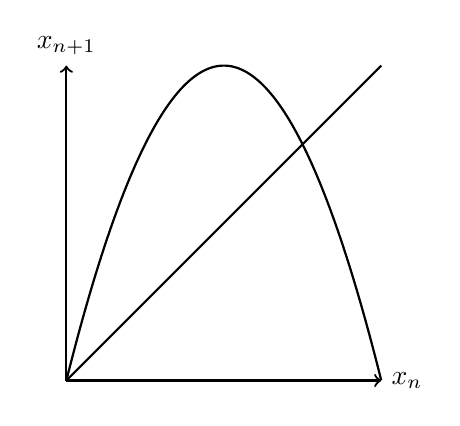
\begin{tikzpicture}
\draw[thick,->] (0,0) -- (4,0) node[right] {$x_n$};
\draw[thick,->] (0,0) -- (0,4) node[above] {$x_{n+1}$};
\draw[thick,domain=0:4,samples=100] plot (\x,{4*\x*(1-\x/4)});
\draw[thick] (0,0) -- (4,4);
\end{tikzpicture}
\caption{Cobweb diagram illustrating the logistic map.}
\end{figure}

\subsection{Bifurcations and Period Doubling}
Bifurcations occur when a small change in $r$ leads to a qualitative change in the system's behavior. Period doubling is a sequence of bifurcations where the periodicity of the system doubles with each step, eventually leading to chaos.

\subsection{Sensitivity to Initial Conditions}
Chaotic systems exhibit extreme sensitivity to initial conditions. Two nearly identical initial states diverge exponentially over time, making long-term predictions impossible.

\subsection{Power Spectrum}
The power spectrum of a chaotic system is broad and continuous, unlike the discrete peaks of a periodic system. This reflects the aperiodic nature of chaos.

\section{Fractal Patterns and Cobweb Graphs}

\subsection{Fractal Patterns}
Chaotic systems often exhibit fractal structures in their phase space. These structures have self-similarity and fractional dimensions, providing insight into the system's complexity.

\subsection{Cobweb Graphs}
A cobweb graph visualizes iterations of a discrete map. Starting from an initial point, a trajectory is plotted using vertical and horizontal lines between the map's function and the diagonal $x_{n+1} = x_n$. This technique highlights fixed points and periodic orbits.

\section{Answers to Questions}

\subsection{Path Crossing in Phase Space}
In an autonomous system, a path in phase space cannot cross itself because the future evolution of the system is uniquely determined by its current state. If a path were to cross, it would imply two different trajectories emerging from the same state, violating the uniqueness of solutions to the differential equations.
The passage explains a fundamental principle in dynamical systems and phase space analysis. In an autonomous system, which does not explicitly depend on time, the evolution of the system is entirely determined by its current state as represented in phase space. Phase space is a conceptual space where all possible states of a system are represented, with each point corresponding to a unique state of the system.

According to this principle, a trajectory or path in phase space cannot intersect itself. If it did, it would indicate that the same state could lead to multiple future developments, contradicting the idea that differential equations governing the system have unique solutions for given initial conditions. Hence, once you know the current state of the system, its future trajectory is fixed and cannot branch into different paths.

\subsection{Solutions for $\frac{d\mathbf{u}}{dt} = A\mathbf{u}$}
For a system $\frac{d\mathbf{u}}{dt} = A\mathbf{u}$, the solutions are of the form:
\[
\mathbf{u}(t) = c_1 e^{\lambda_1 t}\mathbf{v}_1 + c_2 e^{\lambda_2 t}\mathbf{v}_2 + \cdots,
\]
where $\lambda_i$ and $\mathbf{v}_i$ are the eigenvalues and eigenvectors of $A$. The paths in phase space are determined by the nature of the eigenvalues:
\begin{itemize}
  \item Real and distinct eigenvalues: Straight-line trajectories, either converging to or diverging from the origin depending on the sign of $\lambda_i$.
  \item Complex eigenvalues: Spiral trajectories, with the direction of spiraling determined by the sign of the real part of $\lambda_i$.
  \item Repeated eigenvalues: Degenerate behavior, such as parallel trajectories or growth with additional polynomial terms.

\end{itemize}
\usetikzlibrary{decorations.markings}
\tikzset
 {every pin/.style = {pin edge = {<-}},    % pins are arrows from label to point
  > = stealth,                            % arrow tips look like stealth bombers
  flow/.style =    % everything marked as "flow" will be decorated with an arrow
   {decoration = {markings, mark=at position #1 with {\arrow{>}}},
    postaction = {decorate}
   },
  flow/.default = 0.5,          % default position of the arrow is in the middle
  main/.style = {line width=1pt}                    % thick lines for main graph
 }

% \newtemplate[Scaling, default 0.18]{\NameOfTemplate}{Caption}{Code}
\newcommand\newtemplate[4][0.18]%
 {\newsavebox#2%
  \savebox#2%
   {\begin{tabular}{@{}c@{}}
      \begin{tikzpicture}[scale=#1]
      #4
      \end{tikzpicture}\\[-1ex]
      \templatecaption{#3}\\[-1ex]
    \end{tabular}%
   }%
 }
\newcommand\template[1]{\usebox{#1}}             % use the Code stored in box #1
\newcommand\templatecaption[1]{{\sffamily\scriptsize#1}}       % typeset caption
\newcommand\Tr{\mathop{\mathrm{Tr}}}

\newtemplate\sink{sink}%
 {\foreach \sx in {+,-}                   % for right/left half do:
   {\draw[flow] (\sx4,0) -- (0,0);        %   draw half of horizontal axis
    \draw[flow] (0,\sx4) -- (0,0);        %   draw half of vertical axis
    \foreach \sy in {+,-}                 %   for upper/lower quadrant do:
      \foreach \a/\b in {2/1,3/0.44}      %     draw two half-parabolas
        \draw[flow,domain=\sx\a:0] plot (\x, {\sy\b*\x*\x});
   }
 }

\newtemplate\source{source}%
 {\foreach \sx in {+,-}                   % for right/left half do:
   {\draw[flow] (0,0) -- (\sx4,0);        %   draw half of horizontal axis
    \draw[flow] (0,0) -- (0,\sx4);        %   draw half of vertical axis
    \foreach \sy in {+,-}                 %   for upper/lower quadrant do:
      \foreach \a/\b in {2/1,3/0.44}      %     draw two half-parabolas
        \draw[flow,domain=0:\sx\a] plot (\x, {\sy\b*\x*\x});
   }
 }

\newtemplate\stablefp{line of stable fixed points}%
 {\draw (-4,0) -- (4,0);                  % draw horizontal axis
  \foreach \sy in {+,-}                   % for upper/lower half do:
   {\draw[flow] (0,\sy4) -- (0,0);        %   draw half of vertical axis
    \foreach \x in {-3,-2,-1,1,2,3}       %   draw six vertical half-lines
      \draw[flow] (\x,\sy3) -- (\x,0);
   }
 }

\newtemplate\unstablefp{line of unstable fixed points}%
 {\draw (-4,0) -- (4,0);                  % draw horizontal axis
  \foreach \sy in {+,-}                   % for upper/lower half do:
   {\draw[flow] (0,0) -- (0,\sy4);        %   draw half of vertical axis
    \foreach \x in {-3,-2,-1,1,2,3}       %   draw six vertical half-lines
      \draw[flow] (\x,0) -- (\x,\sy3);
   }
 }

\newtemplate\spiralsink{spiral sink}%
 {\draw (-4,0) -- (4,0);                  % draw horizontal axis
  \draw (0,-4) -- (0,4);                  % draw vertical axis
  \draw [samples=100,smooth,domain=27:7]  % draw spiral
       plot ({\x r}:{0.005*\x*\x});       % Using "flow" here gives "Dimension
  \def\x{26}                              %        too large", so we draw a tiny
  \draw[->] ({\x r}:{0.005*\x*\x}) -- +(0.01,-0.01);%     tangent for the arrow.
 }

\newtemplate\spiralsource{spiral source}%
 {\draw (-4,0) -- (4,0);                  % draw horizontal axis
  \draw (0,-4) -- (0,4);                  % draw vertical axis
  \draw [samples=100,smooth,domain=10:28] % draw spiral
       plot ({-\x r}:{0.005*\x*\x});      % Using "flow" here gives "Dimension
  \def\x{27.5}                            %        too large", so we draw a tiny
  \draw[<-] ({-\x r}:{0.005*\x*\x}) -- +(0.01,-0.008);%   tangent for the arrow.
 }

\newtemplate[0.15]\centre{center}% British spelling since \center is in use
 {\draw (-4,0) -- (4,0);                  % draw horizontal axis
  \draw (0,-4) -- (0,4);                  % draw vertical axis
  \foreach \r in {1,2,3}                  % draw three circles
    \draw[flow=0.63] (\r,0) arc (0:-360:\r cm);
 }

\newtemplate\saddle{saddle}%
 {\foreach \sx in {+,-}                   % for right/left half do:
   {\draw[flow] (\sx4,0) -- (0,0);        %   draw half of horizontal axis
    \draw[flow] (0,0) -- (0,\sx4);        %   draw half of vertical axis
    \foreach \sy in {+,-}                 %   for upper/lower quadrant do:
      \foreach \a/\b/\c/\d in {2.8/0.3/0.7/0.6, 3.9/0.4/1.3/1.1}
        \draw[flow] (\sx\a,\sy\b)         %     draw two bent lines
          .. controls (\sx\c,\sy\d) and (\sx\d,\sy\c)
          .. (\sx\b,\sy\a);
   }
 }

\newtemplate\degensink{degenerate sink}%
 {\draw (0,-4) -- (0,4);                  % draw vertical axis
  \foreach \s in {+,-}                    % for upper/lower half do:
   {\draw[flow] (\s4,0) -- (0,0);         %   draw half of horizontal axis
    \foreach \a/\b/\c/\d in {3.5/4/1.5/1, 2.5/2/1/0.8}
      \draw[flow] (\s-3.5,\s\a)           %   draw two bent lines
        .. controls (\s\b,\s\c) and (\s\b,\s\d)
        .. (0,0);
   }
 }

\newtemplate\degensource{degenerate source}%
 {\draw (0,-4) -- (0,4);                  % draw vertical axis
  \foreach \s in {+,-}                    % for upper/lower half do:
   {\draw[flow] (0,0) -- (\s4,0);         %   draw half of horizontal axis
    \foreach \a/\b/\c/\d in {3.5/4/1.5/1, 2.5/2/1/0.8}
      \draw[flow] (0,0)                   %   draw two bent lines
        .. controls (\s\b,\s\d) and (\s\b,\s\c)
        .. (\s-3.5,\s\a);
   }
 }
\begin{document}
\begin{tikzpicture}[line cap=round,line join=round]
  % MAIN DIAGRAM
  \draw [main,->] (0,-0.3) -- (0,4.7)                            % vertical axis
    node [label={[above]$\scriptstyle\det A$}] {}
    node [label={[above,yshift=0.8cm]%
      {\sffamily\large Poincar\'e Diagram: Classification of Phase
      Portraits in the $(\det A,\Tr A)$-plane}}] {};
  \draw [main,->] (-5,0) -- (5,0)                              % horizontal axis
    node [label={[right,yshift=-0.5ex]$\scriptstyle\Tr A$}] {}; 
  \draw [main, domain=-4:4] plot (\x, {0.25*\x*\x});                % main graph
  \node at (-4,4) [pin={[above]$\scriptstyle\Delta=0$}] {};
  \node at ( 4,4) [pin={[above,align=left]%
    {$\scriptstyle\Delta=0:\;\det A=\frac{1}{4}(\Tr A)^2$}}] {};
  % TEMPLATES describing areas
  \node at ( 0  ,-1.4) {\template\saddle};
  \node at (-4  , 1  ) {\template\sink};
  \node at ( 4  , 1  ) {\template\source}; 
  \node at (-1.8, 3.7) {\template\spiralsink};
  \node at ( 1.8, 3.7) {\template\spiralsource};
  % TEMPLATES labeling lines and points
  \node at ( 0  , 1.2) [pin={[draw,right,xshift=0.3cm]%
    \template\centre}] {};
  \node at (-3  , 0  ) [pin={[draw,below,yshift=-1cm]%
    \template\stablefp}] {};
  \node at ( 3  , 0  ) [pin={[draw,below,yshift=-1cm]%
    \template\unstablefp}] {};
  \node at (-3.5,{0.25*3.5*3.5}) [pin={[draw,left,xshift=-1.15cm,yshift=-0.3cm]%
    \template\degensink}] {};
  \node at ( 3.5,{0.25*3.5*3.5}) [pin={[draw,right,xshift=0.9cm,yshift=-0.3cm]%
    \template\degensource}] {};
  \node at ( 0  , 0  ) [pin={[draw,above left,align=center,xshift=-0.3cm]%
    \templatecaption{uniform}\\[-1ex]\templatecaption{motion}}] {};
\end{tikzpicture}

\begin{figure}
    \centering
    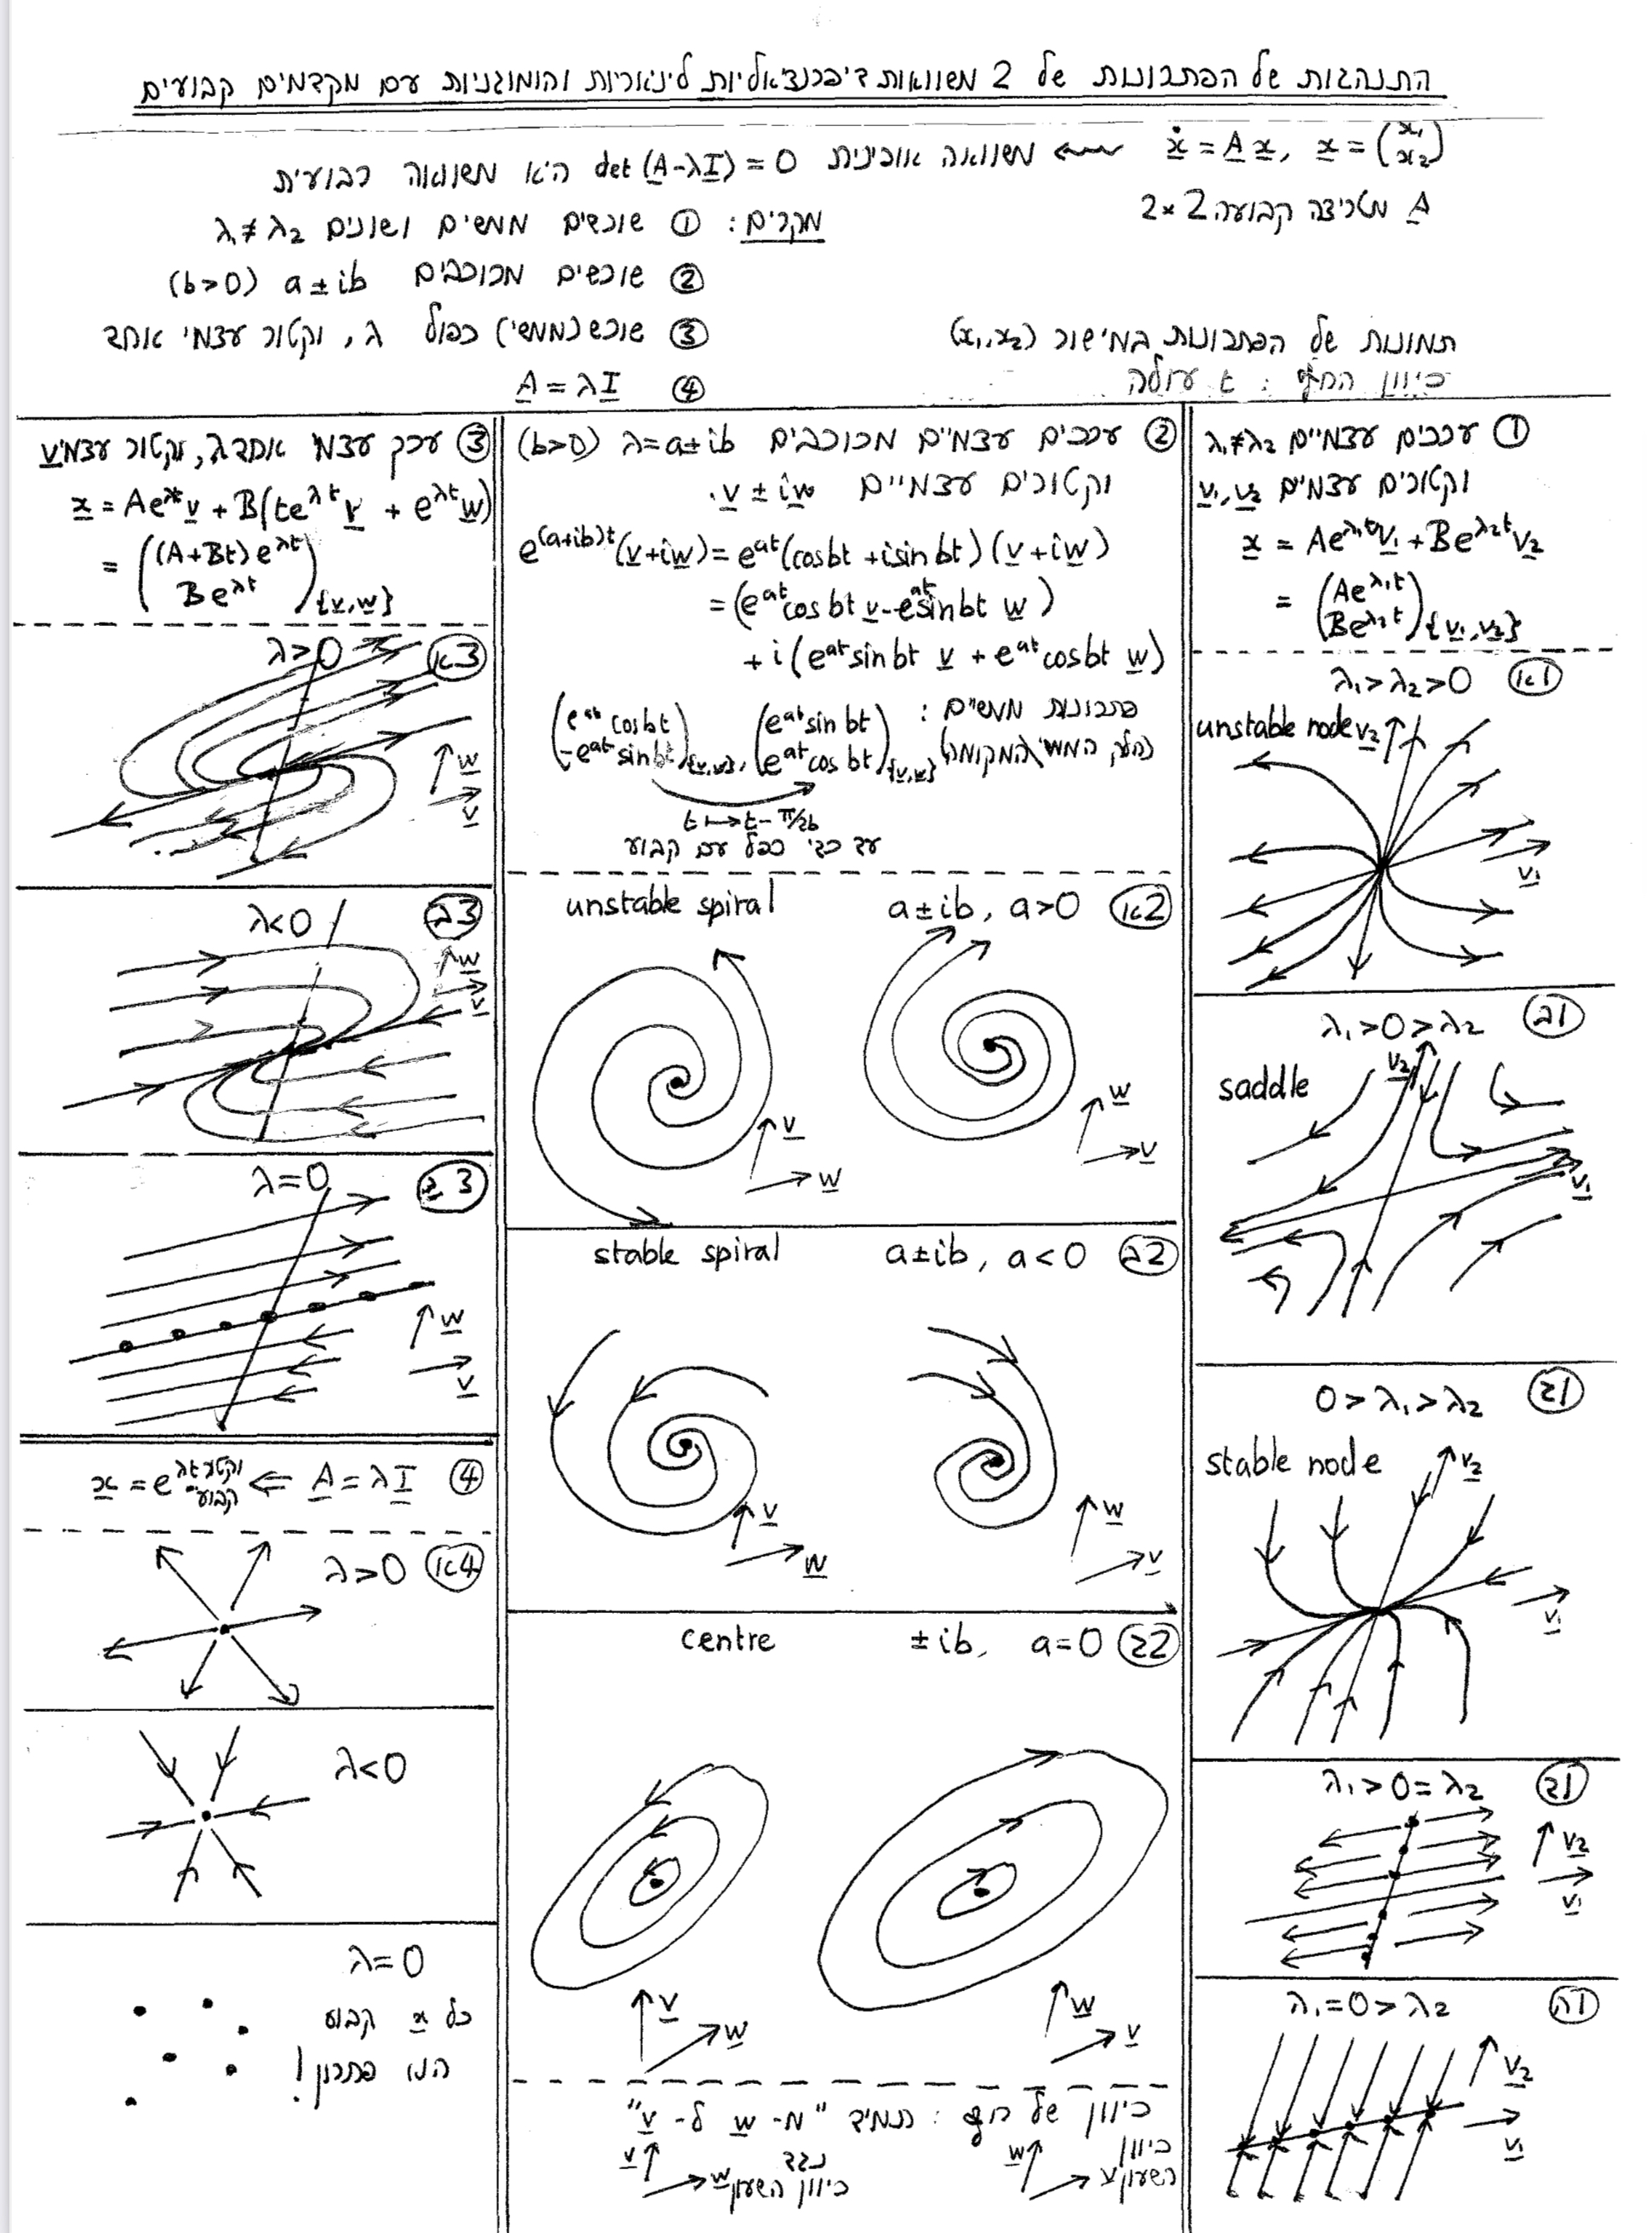
\includegraphics[width=1\linewidth]{Screenshot 2024-12-18 at 12.52.22.jpg}
    \caption{Enter Caption}
    \label{fig:enter-label}
\end{figure}

\subsection{Repeated Eigenvalues}
When the eigenvalues of $A$ are identical, the system might not possess sufficient independent eigenvectors to construct a comprehensive basis. This situation gives rise to generalized eigenvectors and non-diagonalizable characteristics, leading to solutions that feature polynomial terms in $t$ together with exponential terms.

\begin{center}
\setlength{\fboxsep}{10pt}
\fbox{
    \begin{minipage}{0.9\textwidth}
        \textbf{Poincaré Section for Different Paths:}

        A Poincaré section samples the trajectory of a dynamical system at regular intervals in phase space, reducing its dimensionality. Here's how the Poincaré section appears for various paths:

        \begin{enumerate}
            \item \textbf{Fixed Point:}
            \begin{itemize}
                \item \textbf{Path Description:} The system's trajectory remains stationary, representing an equilibrium in phase space.
                \item \textbf{Appearance in Poincaré Section:} A single point, as the trajectory intersects the same location repeatedly.
            \end{itemize}

            \item \textbf{Periodic Path:}
            \begin{itemize}
                \item \textbf{Path Description:} The trajectory forms a closed loop in phase space, repeating after a finite period.
                \item \textbf{Appearance in Poincaré Section:} A finite set of distinct points arranged in a closed pattern, each corresponding to an intersection of the trajectory with the Poincaré plane during one period.
            \end{itemize}

            \item \textbf{Non-Periodic Path:}
            \begin{itemize}
                \item \textbf{Path Description:} The trajectory does not repeat, exhibiting chaotic or quasi-periodic behavior.
                \item \textbf{Appearance in Poincaré Section:}
                \begin{itemize}
                    \item \textbf{Chaotic Path:} A scattered set of points forming a fractal-like structure, reflecting sensitivity to initial conditions and irregular dynamics.
                    \item \textbf{Quasi-Periodic Path:} A dense set of points forming a smooth curve, representing non-repeating but smooth behavior.
                \end{itemize}
            \end{itemize}
        \end{enumerate}
    \end{minipage}
}
\end{center}

\end{itemize}

\subsection{Stability Condition for Fixed Points}
The condition $|f'_r(x^*)| < 1$ dictates the stability of a fixed point in a discrete map. This criterion guarantees that minor disturbances reduce over successive iterations, thus maintaining the system's proximity to the fixed point.

\subsection{Logistic Map and Population Growth}
The logistic map characterizes population dynamics considering competition via the following expressions:
\begin{itemize}
  \item $r x_n$: Indicates the exponential increase attributed to reproduction processes.
  \item $-r x_n^2$: Accounts for the competition over scarce resources, thereby curtailing growth.
\end{itemize}
The parameter $r$ dictates not only the pace of growth but also the strength of competitive interactions, thus shaping the behavior of the population over time.

\subsection{Logistic Map and Behavior for $r$}
\begin{center}
\setlength{\fboxsep}{10pt}
\fbox{
    \begin{minipage}{0.9\textwidth}
        \textbf{Why Does \( r \) Determine the Nonlinearity of the Logistic Map Equation?}

        In the logistic map:
        \[
        x_{n+1} = r x_n (1 - x_n),
        \]
        we can rewrite the equation as:
        \[
        x_{n+1} = r x_n - r x_n^2.
        \]

        The parameter \( r \) directly influences the degree of nonlinearity in the equation because it scales both the linear and nonlinear terms. Here's how:

        \begin{enumerate}
            \item \textbf{Linear Term (\( r x_n \)):}
            \begin{itemize}
                \item This term represents exponential growth in the population, driven solely by reproduction.
                \item The coefficient \( r \) amplifies or diminishes the overall growth rate.
            \end{itemize}

            \item \textbf{Nonlinear Term (\( -r x_n^2 \)):}
            \begin{itemize}
                \item This term introduces competition due to limited resources. As the population increases, the term \( x_n^2 \) becomes significant, slowing growth.
                \item The factor \( r \) determines the strength of this competition, making it proportional to the growth rate.
            \end{itemize}
        \end{enumerate}

        \textbf{Why Does \( r \) Influence Nonlinearity?}
        Since \( r \) multiplies both the linear term (\( x_n \)) and the nonlinear term (\( x_n^2 \)), increasing \( r \) amplifies the influence of the nonlinear term relative to the linear one. For large values of \( r \), the nonlinearity dominates, leading to complex dynamics such as bifurcations and chaos.

        In summary, \( r \) controls both the growth rate and the intensity of competition, determining the balance between linear and nonlinear effects in the system.
    \end{minipage}
}
\end{center}

\begin{center}
\setlength{\fboxsep}{10pt}
\fbox{
    \begin{minipage}{0.9\textwidth}
        \textbf{Behavior of the Logistic Map for \( 0 \leq r \leq 3 \) and Why the Proof Fails for \( r > 3 \):}

        The logistic map is defined as:
        \[
        x_{n+1} = r x_n (1 - x_n),
        \]
        where \( x_n \) represents the population normalized between 0 and 1, and \( r \) is the growth rate parameter.

        \textbf{Behavior for \( 0 \leq r \leq 3 \):}
        \begin{itemize}
            \item For \( 0 < r < 1 \):
            \begin{itemize}
                \item The population decreases exponentially to zero (\( x_n \to 0 \)) because the growth rate is too small to sustain the population.
            \end{itemize}
            \item For \( 1 \leq r < 3 \):
            \begin{itemize}
                \item The population converges to a stable fixed point \( x^* \), which can be found by solving:
                \[
                x^* = r x^* (1 - x^*).
                \]
                Rearranging gives:
                \[
                x^* = 1 - \frac{1}{r}.
                \]
                This fixed point is stable as long as \( r \leq 3 \), because perturbations in \( x_n \) decay over time.
            \end{itemize}
        \end{itemize}

        \textbf{Why the Proof Fails for \( r > 3 \):}
        \begin{itemize}
            \item For \( r > 3 \), the fixed point \( x^* = 1 - \frac{1}{r} \) becomes unstable. Small perturbations around \( x^* \) grow instead of decaying, leading to:
            \begin{itemize}
                \item **Periodic Behavior:** Oscillations between two or more points (period-doubling bifurcations).
                \item **Chaotic Behavior:** For \( r > 3.57 \), the trajectory becomes aperiodic and unpredictable, sensitive to initial conditions.
            \end{itemize}
            \item The failure occurs because the condition for stability:
            \[
            |f'(x^*)| < 1,
            \]
            is violated. For \( r > 3 \), the derivative of the map at the fixed point \( f'(x^*) = r (1 - 2x^*) \) exceeds 1, leading to instability.
        \end{itemize}

        \textbf{Conclusion:}
        For \( 0 \leq r \leq 3 \), the logistic map exhibits stable behavior, but for \( r > 3 \), the system transitions to periodic or chaotic dynamics due to the instability of the fixed point.
    \end{minipage}
}
\end{center}


\subsection{Fixed Points of $f_4(x)$}
\begin{center}
\setlength{\fboxsep}{10pt}
\fbox{
    \begin{minipage}{0.9\textwidth}
        \textbf{Proof that \( f_4(x) \) Has a Fixed Point in \( \left[ 0, \frac{1}{2} \right] \):}

        The function \( f_4(x) \) is defined as:
        \[
        f_4(x) = f(f(f(f(x)))) = f^{(4)}(x),
        \]
        where \( f(x) = r x (1 - x) \) is the logistic map.

        \textbf{Key Properties of \( f_4(x) \):}
        \begin{enumerate}
            \item \( f_4(x) \) is continuous on the interval \( \left[ 0, \frac{1}{2} \right] \).
            \item The logistic map \( f(x) = r x (1 - x) \) maps \( \left[ 0, 1 \right] \) into itself, so \( f_4(x) \) also maps \( \left[ 0, \frac{1}{2} \right] \) into \( \left[ 0, 1 \right] \).
        \end{enumerate}

        \textbf{Intermediate Value Theorem:}
        To show the existence of a fixed point \( x^* \) where \( f_4(x^*) = x^* \) in \( \left[ 0, \frac{1}{2} \right] \), consider the function:
        \[
        g(x) = f_4(x) - x.
        \]
        \begin{itemize}
            \item \( g(x) \) is continuous because \( f_4(x) \) is continuous.
            \item At the endpoints of the interval:
            \[
            g(0) = f_4(0) - 0 = 0 - 0 = 0,
            \]
            \[
            g\left(\frac{1}{2}\right) = f_4\left(\frac{1}{2}\right) - \frac{1}{2}.
            \]
            Depending on \( r \), \( g\left(\frac{1}{2}\right) \) may be positive or negative. Since \( f_4(x) \) maps \( \left[ 0, \frac{1}{2} \right] \) into itself, \( g(x) \) will take on both positive and negative values within the interval.
        \end{itemize}

        \textbf{Application of the Intermediate Value Theorem:}
        Since \( g(x) \) is continuous and \( g(0) = 0 \), while \( g\left(\frac{1}{2}\right) \) can be negative or positive:
        \begin{itemize}
            \item By the Intermediate Value Theorem, there exists at least one \( x^* \in \left[ 0, \frac{1}{2} \right] \) such that:
            \[
            g(x^*) = f_4(x^*) - x^* = 0,
            \]
            or equivalently:
            \[
            f_4(x^*) = x^*.
            \]
        \end{itemize}

        \textbf{Conclusion:}
        \( f_4(x) \) has at least one fixed point \( x^* \) in \( \left[ 0, \frac{1}{2} \right] \), guaranteed by the Intermediate Value Theorem and the properties of the logistic map.
    \end{minipage}
}
\end{center}

To show that $f_4(x)$ has a fixed point in the interval $\left[ 0, \frac{1}{2} \right]$, consider the iterative process of solving $f_4(x) = x$. Computational tools like Mathematica confirm a fixed point exists in this interval.


\subsection{Fixed Points of $h = g^2 = f^4$}
Using software, we compute the fixed points of $h = g^2 = f^4$ and their stability. In the range $3.45 \leq r \leq 3.54$, the system displays a periodic orbit of length 4, confirmed by bifurcation diagrams and stability analysis.
\begin{figure}
    \centering
    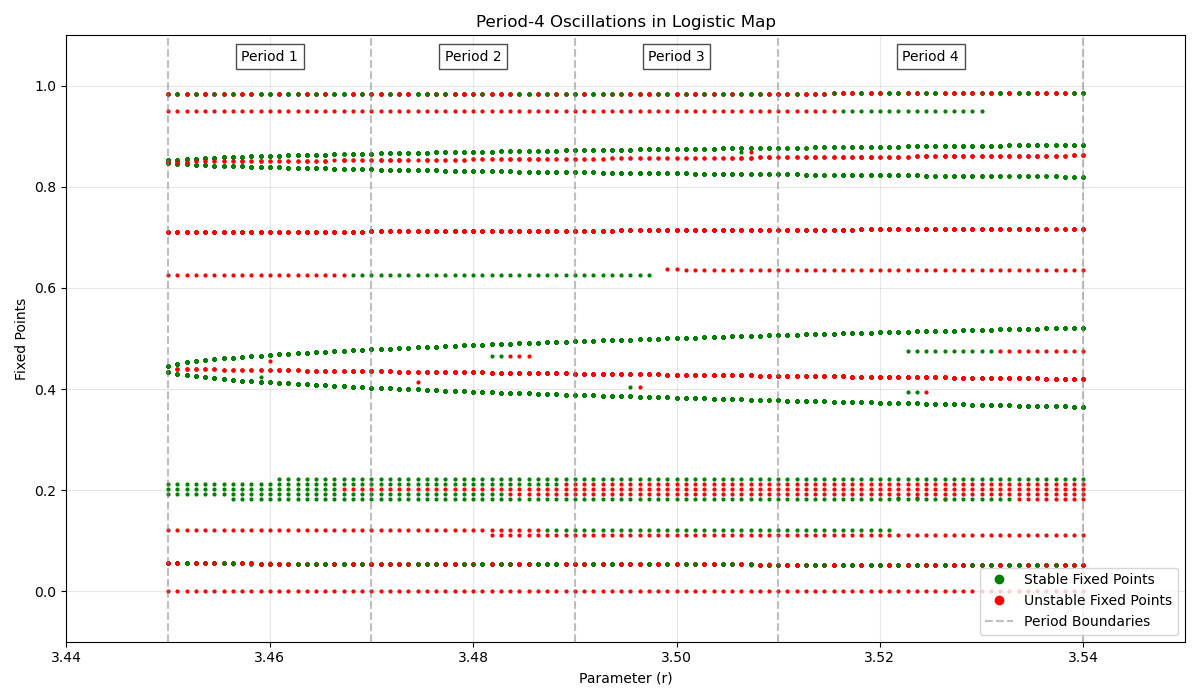
\includegraphics[width=1\linewidth]{Figure_1.png}
   Fixed Points of  $h = g^2 = f^4$}
    \label{fig:enter-label}
\end{figure}
\begin{figure}
    \centering
    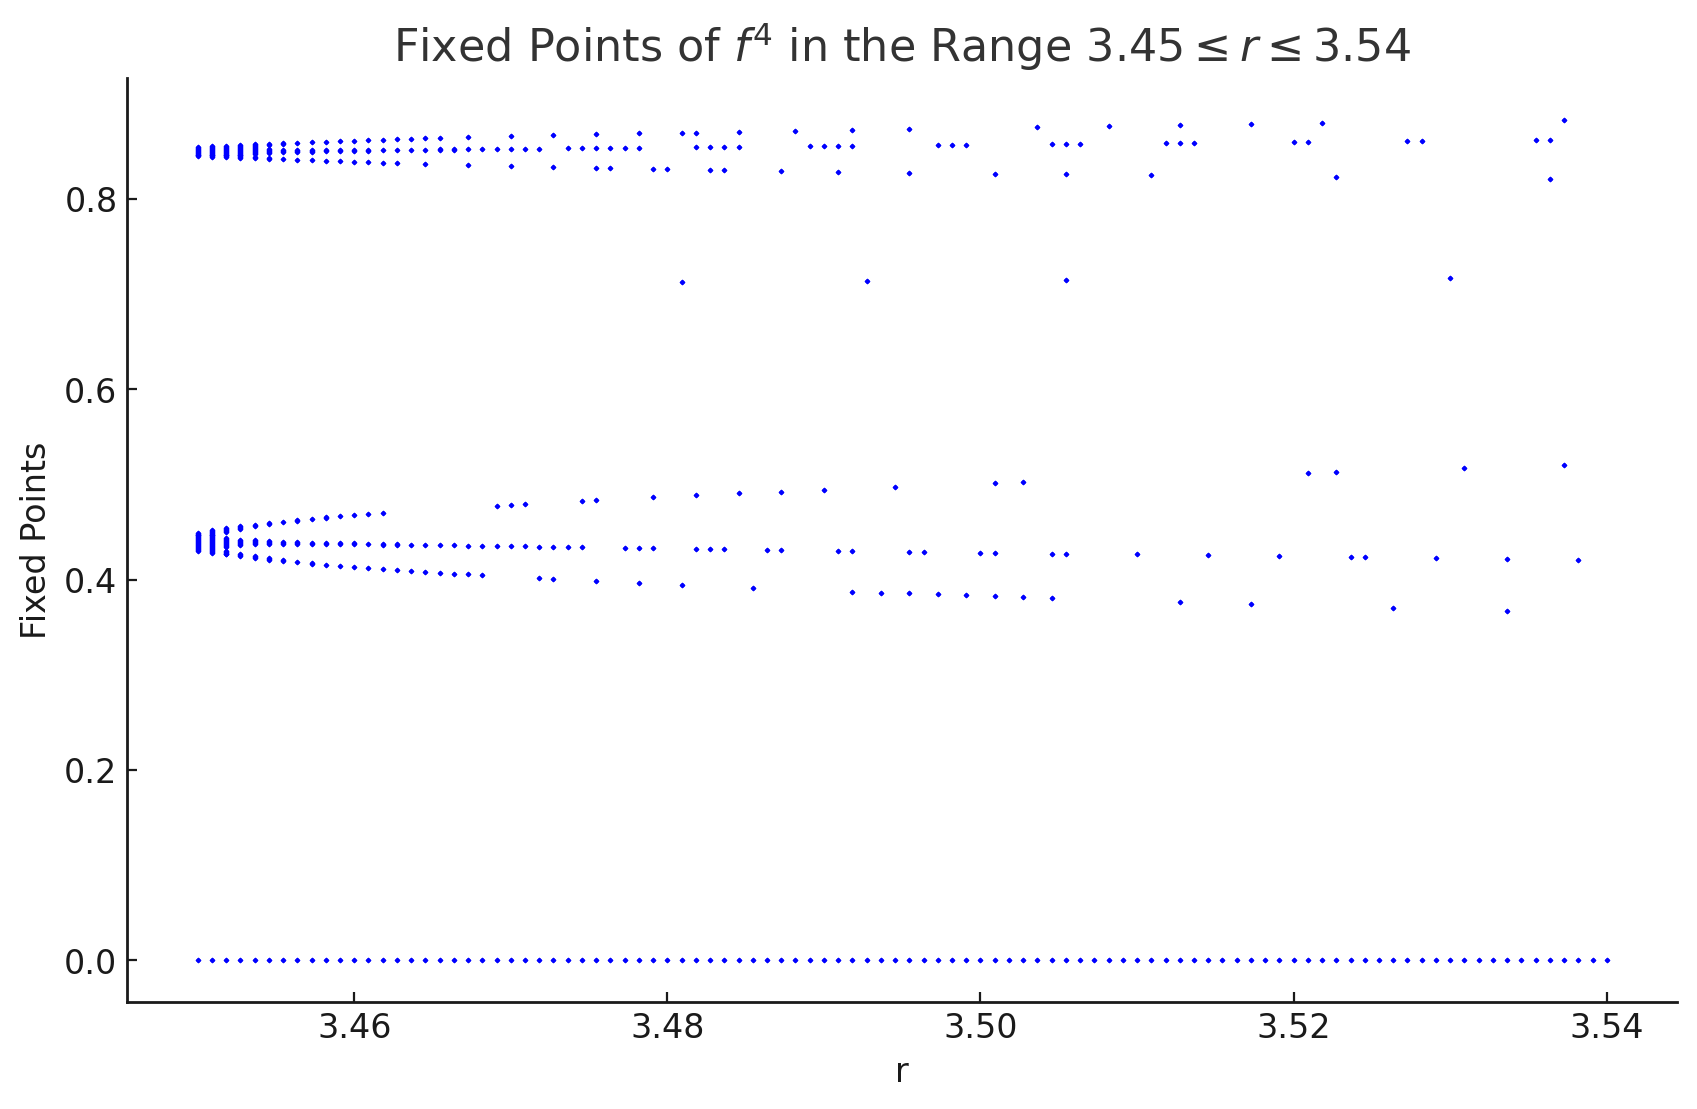
\includegraphics[width=1\linewidth]{image.png}
    \caption{Fixed Points of  $h = g^2 = f^4$ }
    \label{fig:enter-label}
\end{figure}

\subsection{Fixed Point of $f_4(x)$ in $[0, 1/2]$}
To show that $f_4(x)$ has a fixed point in $[0, 1/2]$, consider the iteration $f_4(x) = f(f(f(f(x))))$. Using intermediate value theorem arguments and the bounded nature of $f(x)$, there must be at least one fixed point in the interval.

\subsection{Periodic Orbit of Length 4 for $3.45 \leq r \leq 3.54$}
Using computational tools like Mathematica, compute the fixed points of $g^2 = f^4$ in the range $3.45 \leq r \leq 3.54$. The results show that the system undergoes period-4 oscillations, with stability determined by evaluating $|f'_r(x)|$ at each fixed point.Fourier Transform of Chaotic Systems
A chaotic system without a fixed period exhibits a continuous, broad-spectrum Fourier transform due to the aperiodic nature of its dynamics. This differs from a system with period-doubling, where the Fourier spectrum contains discrete peaks at harmonics of the fundamental frequency.

        \textbf{Difference Between Harmonics and Period-Doubling:}

        \textbf{1. Harmonics:}
        \begin{itemize}
            \item When a periodic but non-sinusoidal signal is introduced into a linear system, the system's response includes harmonic frequencies.
            \item These harmonics are integer multiples of the fundamental frequency of the input signal, such as \( f, 2f, 3f, \dots \).
            \item Harmonics arise from the Fourier decomposition of the non-sinusoidal signal. Each harmonic corresponds to a sinusoidal component of the original signal.
            \item The presence of harmonics is a linear phenomenon and does not indicate a change in the system's intrinsic behavior.
        \end{itemize}

        \textbf{2. Period-Doubling:}
        \begin{itemize}
            \item Period-doubling occurs in nonlinear systems when a parameter (e.g., \( r \) in the logistic map) changes, causing the system's behavior to shift from a single period to oscillations with double the period.
            \item This is not related to the input signal but instead represents a bifurcation in the system's dynamics.
            \item Period-doubling is a precursor to chaos. It is characterized by frequencies such as \( f, f/2, f/4, \dots \), indicating increasingly long oscillation periods.
            \item Unlike harmonics, period-doubling reflects a qualitative change in the system's behavior due to nonlinearity.
        \end{itemize}

        \textbf{Key Differences:}
        \begin{itemize}
            \item \textbf{Source:} Harmonics result from the input signal's structure, while period-doubling arises from intrinsic nonlinear dynamics.
            \item \textbf{Frequencies:} Harmonics are integer multiples of the fundamental frequency, whereas period-doubling involves subharmonic frequencies (fractions of the fundamental frequency).
            \item \textbf{System Behavior:} Harmonics do not change the system's behavior, while period-doubling indicates a transition toward chaotic dynamics.
        \end{itemize}

        \textbf{Conclusion:}
        Harmonics reflect the decomposition of a periodic input signal in a linear system, while period-doubling is a nonlinear phenomenon signaling a qualitative shift in the system's dynamics.
        
\begin{center}
    \begin{minipage}{0.9\textwidth}
        \textbf{Oscilloscope Measurements: Sampling Rate and Observation Time}

        \textbf{1. Key Factors in Oscilloscope Measurements:}
        \begin{itemize}
            \item \textbf{Sampling Rate (\( f_{\text{sampling}} \)):}
            \begin{itemize}
                \item Determines the temporal resolution of the measurements.
                \item Higher sampling rates are necessary to accurately capture fast-changing signals or high-frequency components.
                \item According to the Nyquist theorem, the sampling rate must be at least twice the highest frequency present in the signal to avoid aliasing.
            \end{itemize}

            \item \textbf{Observation Time (\( T_{\text{observation}} \)):}
            \begin{itemize}
                \item Defines the total duration over which the signal is recorded.
                \item Longer observation times are required to analyze slow or long-term dynamics, such as periodic oscillations or transient behaviors.
                \item Observation time affects the resolution in the frequency domain: longer times improve the frequency resolution.
            \end{itemize}
        \end{itemize}

        \textbf{2. Trade-off Between Sampling Rate and Observation Time:}
        The total number of measurements the oscilloscope can record is limited by:
        \[
        N_{\text{measurements}} = f_{\text{sampling}} \cdot T_{\text{observation}}.
        \]
        Increasing \( f_{\text{sampling}} \) reduces \( T_{\text{observation}} \), and vice versa. The choice depends on the nature of the signal:
        \begin{itemize}
            \item For high-frequency or rapidly changing signals, prioritize a high sampling rate to avoid aliasing.
            \item For low-frequency or long-term dynamics, prioritize a longer observation time to capture the full signal evolution.
        \end{itemize}

        \textbf{3. Optimal Combination:}
        To choose the optimal combination:
        \begin{itemize}
            \item Estimate the highest frequency in the signal (\( f_{\text{max}} \)) and set \( f_{\text{sampling}} \geq 2 f_{\text{max}} \).
            \item Ensure \( T_{\text{observation}} \) is sufficient to capture the phenomena of interest, such as multiple periods for periodic signals or complete transient behaviors.
            \item Balance \( f_{\text{sampling}} \) and \( T_{\text{observation}} \) based on the oscilloscope's memory capacity and the specific dynamics being studied.
        \end{itemize}

        \textbf{Conclusion:}
        The optimal combination of sampling rate and observation time depends on the signal characteristics:
        \begin{itemize}
            \item For high-frequency chaotic signals, prioritize high sampling rates.
            \item For low-frequency or long-term signals, prioritize longer observation times.
        \end{itemize}
        Carefully balancing these factors ensures accurate and comprehensive data capture.
    \end{minipage}
\end{center}
\end{document}
